\section{Ideen und Konzepte}
\label{sec:ideen-und-konzepte}

In diesem Kapitel wird aufgezeigt, wie sich die im vorherigen Kapitel erarbeiteten technischen Grundlagen zu einem Design für einen Prototyp zusammenfügen lassen. Hierzu sollen verschiedene Architekturvarianten aufgezeigt und miteinander verglichen werden, von der dann die geeignetste für die Umsetzung vorgeschlagen wird.

\subsection{Architekturvarianten}
\label{sec:architekturvarianten}

Soll für die Schnittstelle nach aussen HTTP verwendet werden (siehe \secref{sec:web-services}), gibt es für die interne Kommunikation zwischen den Komponenten keine expliziten Einschränkungen. Die äussere Schnittstelle gibt jedoch einen Rahmen vor.

Ein wichtiges Merkmal von HTTP ist, dass Anfragen atomar sind, d.h. nur als Ganzes beantwortet werden können: Zu jedem Request gibt es genau eine Response, und jede Response hat genau einen Status-Code, der über den Erfolg bzw. Misserfolg der Anfrage Auskunft gibt.\footnote{Auch wenn ein Status-Code wie \texttt{206 Partial Content} auf die Unvollständigkeit der Antwort hinweist, muss für den Zugriff auf die weiteren Antwortteile wieder ein neuer Request abgesetzt werden \cite[Kapitel 4.1]{RFC7233}.}

Da HTTP ein synchrones Protokoll ist, sollten Anfragen schnell beantwortet werden, d.h. eher in Sekunden (besser Millisekunden) als in Minuten. Dauert eine Anfrage zu lange, wird diese von einem «ungeduldigen» Client abgebrochen. Zwar kann diese Zeitspanne mittels Keep-Alive-Header ausgedehnt werden \cite[Anhang 1.2]{RFC7230}. Dies stellt jedoch Anforderungen an den Client, wessen Konfiguration sich der Hoheit des zu erstellenden Prototyps entzieht.

Eine Batch-Verarbeitung, bei der mehrere Bilder mit einer Anfrage zum Scoring in Auftrag gegeben werden, ist aus diesen beiden Grüden ‒ Atomizität und synchrone Kommunikation ‒ nicht sinnvoll, und soll deshalb nicht angeboten werden. Die RESTful-API soll darauf ausgelegt werden, nur ein Bild pro Request zu verarbeiten. Weiter soll der Prototyp den Anspruch haben, dass einzelne Bilder trotz der vielschichtigen Verarbeitung in einer für einen synchronen Client nützlichen Frist verarbeitet werden.

Die äussere Schnittstelle schliesst somit eine Batch-Verarbeitung aus. Der Protoyp erhält jeweils ein Bild pro Anfrage und soll damit mit einem möglichst vollständigen Scoring antworten, d.h. mit zehn Scores für die einzelnen Gelenke MCP 1-5 und PIP 1-5, sofern es sich beim Bild um eine Röntgenaufnahme einer linken Hand handelt.

Kann das Bild nicht oder nur teilweise verarbeitet werden ‒ sei es aufgrund eines falschen Bildes (keine Röntgenaufnahme oder Röntgenaufnahme eines anderen Körperteils), aufgrund einer schlechten Bildqualität der Röntgenaufnahme, oder aufgrund einer mangelhaftgen Prediction-Performance der involvierten Modelle ‒ sollen zumindest alle ermittelten Scores oder entsprechende Fehlermeldungen zurückgegeben werden.\footnote{Die Wahl der geeigneten HTTP-Status-Codes ist Teil der Implementierung und soll an dieser Stelle nicht weiter besprochen werden.}

Auf Basis der vorgängig diskutierten Integrationsvarianten (siehe \secref{sec:integrationsvarianten}) werden im Folgenden verschiedene Architekturen für die Umsetzung des Prototyps vorgestellt. Dabei wird jeweils von einem Client ausgegangen, der synchron per HTTP mit dem zu erstellenden System (\textit{DeepXRay}) kommuniziert.

\subsubsection{Variante 1: HTTP, synchron}

Die erste Variante (\textit{HTTP, synchron}) verwendet vier verschiedene Komponenten. Dies sind einerseits Komponenten basierend auf den bereits beschriebenen Machine-Learning-Mo\-dellen \texttt{body\_part}, \texttt{joint\_detection} und \texttt{ratingen\_score}.\footnote{Diese Bezeichnungen werden im Folgenden sowohl für die eigentlichen Modelle als auch für die \textit{Modellkomponenten} verwendet, die das jeweilige Modell beinhalten, dieses aber um Integrationscode erweitern. Ob das Modell oder die Modellkomponente gemeint ist, ergibt sich dabei aus dem Kontext.} Andererseits kommt der sogenannte \texttt{orchestrator} hinzu, der für die Kommunikation mit dem Client verantwortlich ist, und die Arbeit der Modellkomponenten koordiniert.

\begin{figure}[tbh]
    \centering
    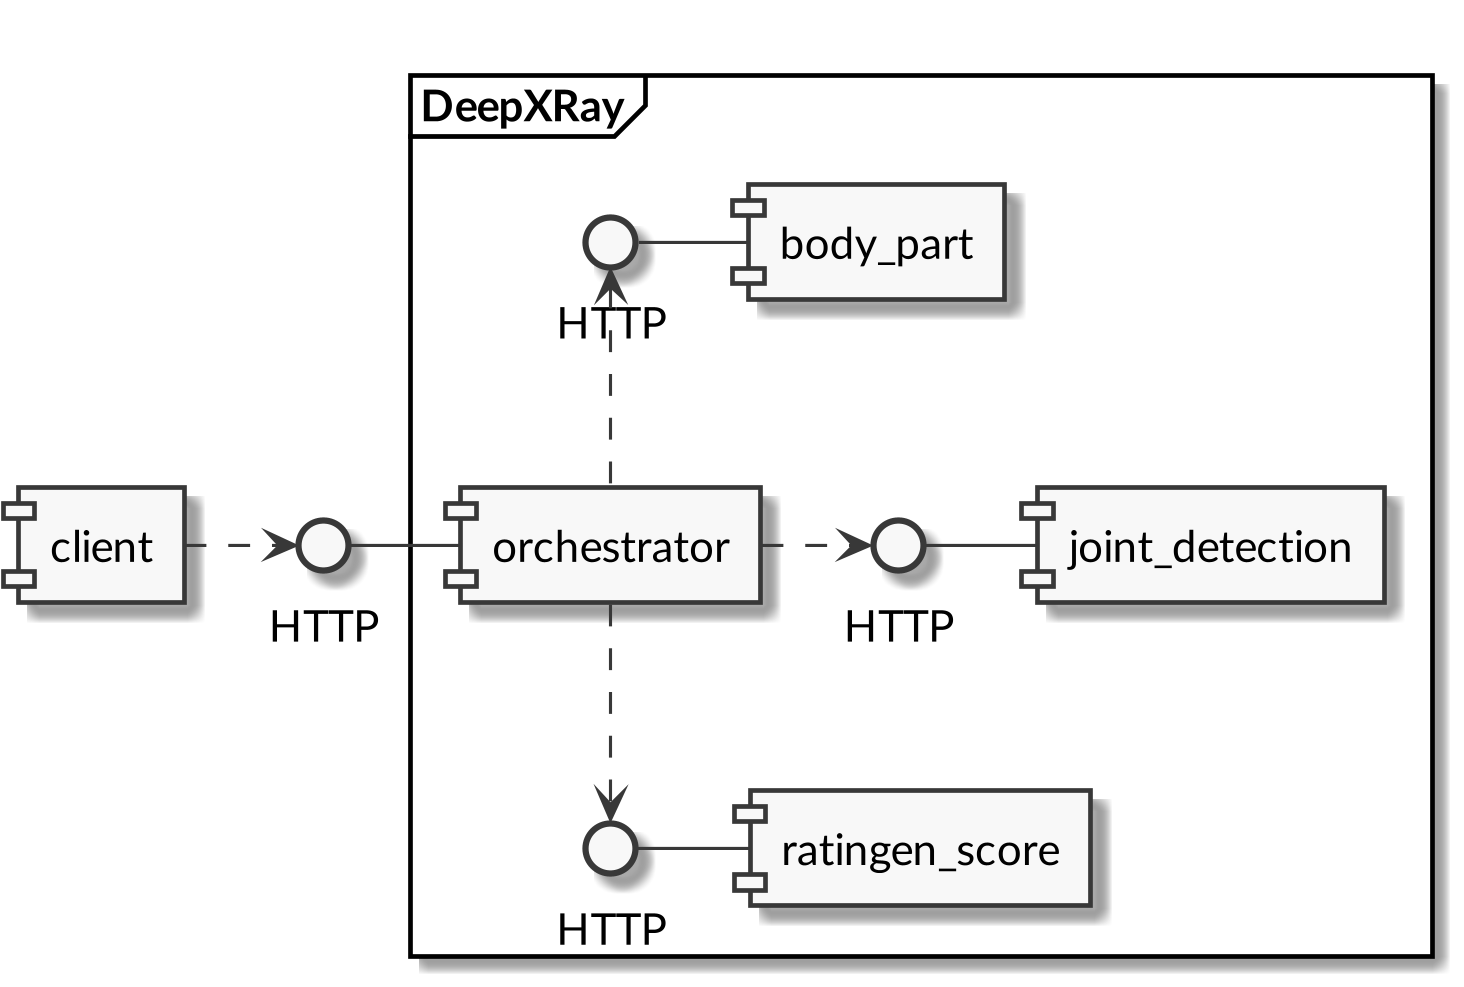
\includegraphics[width=\linewidth]{pics/architektur-variante-http.png}
    \caption{Komponentenarchitektur der Varianten 1 und 2 (HTTP, synchron und synchron/asynchron). Die Modellkomponenten bieten eine HTTP-Schnittstelle an, die vom \texttt{orchestrator} angesprochen wird. (Komponentendiagramm)}
    \label{fig:architektur-variante-http}
\end{figure}

Die Komponentenarchitektur dieser Variante ist auf \imgref{fig:architektur-variante-http} (Komponentendiagramm) ersichtlich. Die drei Modellkomponenten bieten jeweils eine interne HTTP-Schnittstelle an, die vom \texttt{orchestrator} angesprochen werden kann. Zwischen den Modellkomponenten findet keine Kommunikation statt.

\begin{figure}[tbh]
    \centering
    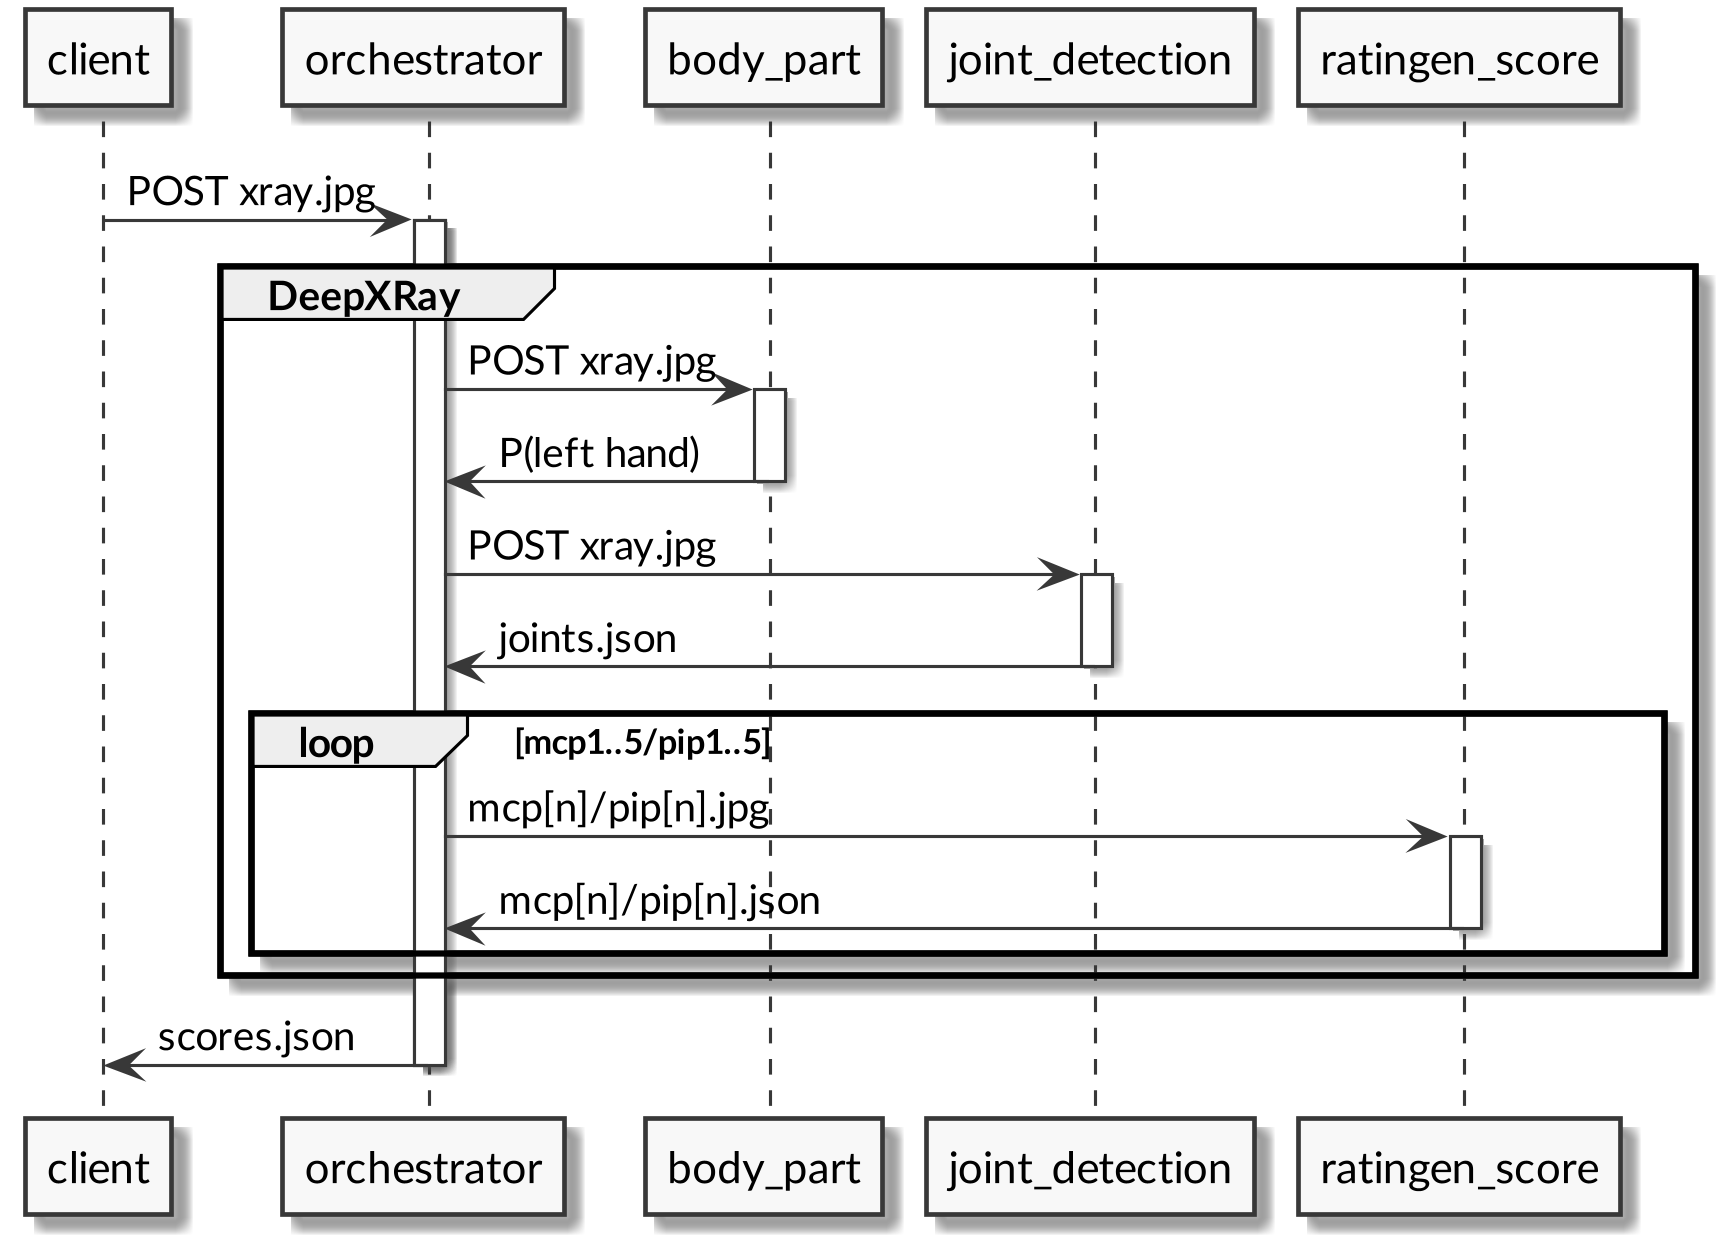
\includegraphics[width=\linewidth]{pics/datenfluss-variante-http-1.png}
    \caption{Datenfluss der Variante 1 (HTTP, synchron). Die einzelnen Modellkomponenten werden streng synchron aufgerufen und sequenziell abgearbeitet. (Sequenzdiagramm)}
    \label{fig:datenfluss-variante-http-1}
\end{figure}

Das Sequenzdiagramm \imgref{fig:datenfluss-variante-http-1} veranschaulicht den Ablauf. Zunächst stellt der \texttt{client} eine HTTP-\texttt{POST}-Anfrage an den \texttt{orchestrator}, welche ein Röntgenbild (\texttt{xray}) enthält. Der \texttt{orchestrator} leitet das Bild weiter zu \texttt{body\_part}. Diese Komponente antwortet mit einer Wahrscheinlichkeit, mit der es sich beim dargestellten Körperteil um eine linke Hand handelt.

Fällt diese Wahrscheinlichkeit genügend hoch aus, um eine Weiterverarbeitung zu rechtfertigen, wird das Röntgenbild weiter an die Komponente \texttt{joint\_detection} gesendet.\footnote{Auf Negativfälle wird in diesem Kapitel nur eingegangen, wo sie für die Konzeption der Architektur ausschlaggebend sind. Ansonsten wird zugunsten der Übersichtlichkeit auf deren Besprechung verzichtet. Negativfälle werden im Kapitel \secref{sec:realisierung} behandelt.} Dort werden die zehn relevanten Gelenke extrahiert und als Bildausschnitte in einem geeigneten Format\footnote{z.B. base64-codiert in einem JSON-Payload} an den \texttt{orchestrator} zurückgeliefert.

Der \texttt{orchestrator} sendet diese extrahierten Bildausschnitte der Reihe nach an die Komponente \texttt{ratingen\_score}, welche das Scoring der dargestellten Gelenke vornimmt. Die Score wird wiederum in einem geeigneten Format an den \texttt{orchestrator} zurückgesendet.

Am Schluss sammelt der \texttt{orchestrator} diese Scores, fasst sie in einer Datenstruktur zusammen, und sendet sie dem Client in einem geeigneten Format (JSON) zurück.

Diese Variante hat folgende Vor- und Nachteile:

\begin{description}
    \item[Vorteile] Die Variante ist sehr einfach umzusetzen. Da HTTP als externe Schnittstelle bereits gesetzt ist, können die internen Schnittstellen den gleichen Ansatz verwenden, wodurch nur eine Art von Schnittstelle benötigt wird.
    \item[Nachteile] Die Extraktion der Gelenke muss abgewartet werden, bis zum Scoring derselben übergegangen werden kann. Das Scoring findet streng sequenziell statt und ist daher langsam. Zu einem bestimmten Zeitpunkt kann jeweils nur eine Instanz der Modellkomponenten genutzt werden.
\end{description}

\subsubsection{Variante 2: HTTP, synchron und asynchron}

Die zweite Variante geht von der gleichen Komponentenarchitektur aus wie die erste Variante, siehe \imgref{fig:architektur-variante-http} (Komponentendiagramm). Im Gegensatz zur ersten Variante soll die zweite Variante jedoch nicht streng synchron arbeiten. Hierzu ändert sich die interne Arbeitsweise der \texttt{orchestrator}-Komponente und die Schnittstelle zur Komponente \texttt{joint\_detection}.

\begin{figure}[tbh]
    \centering
    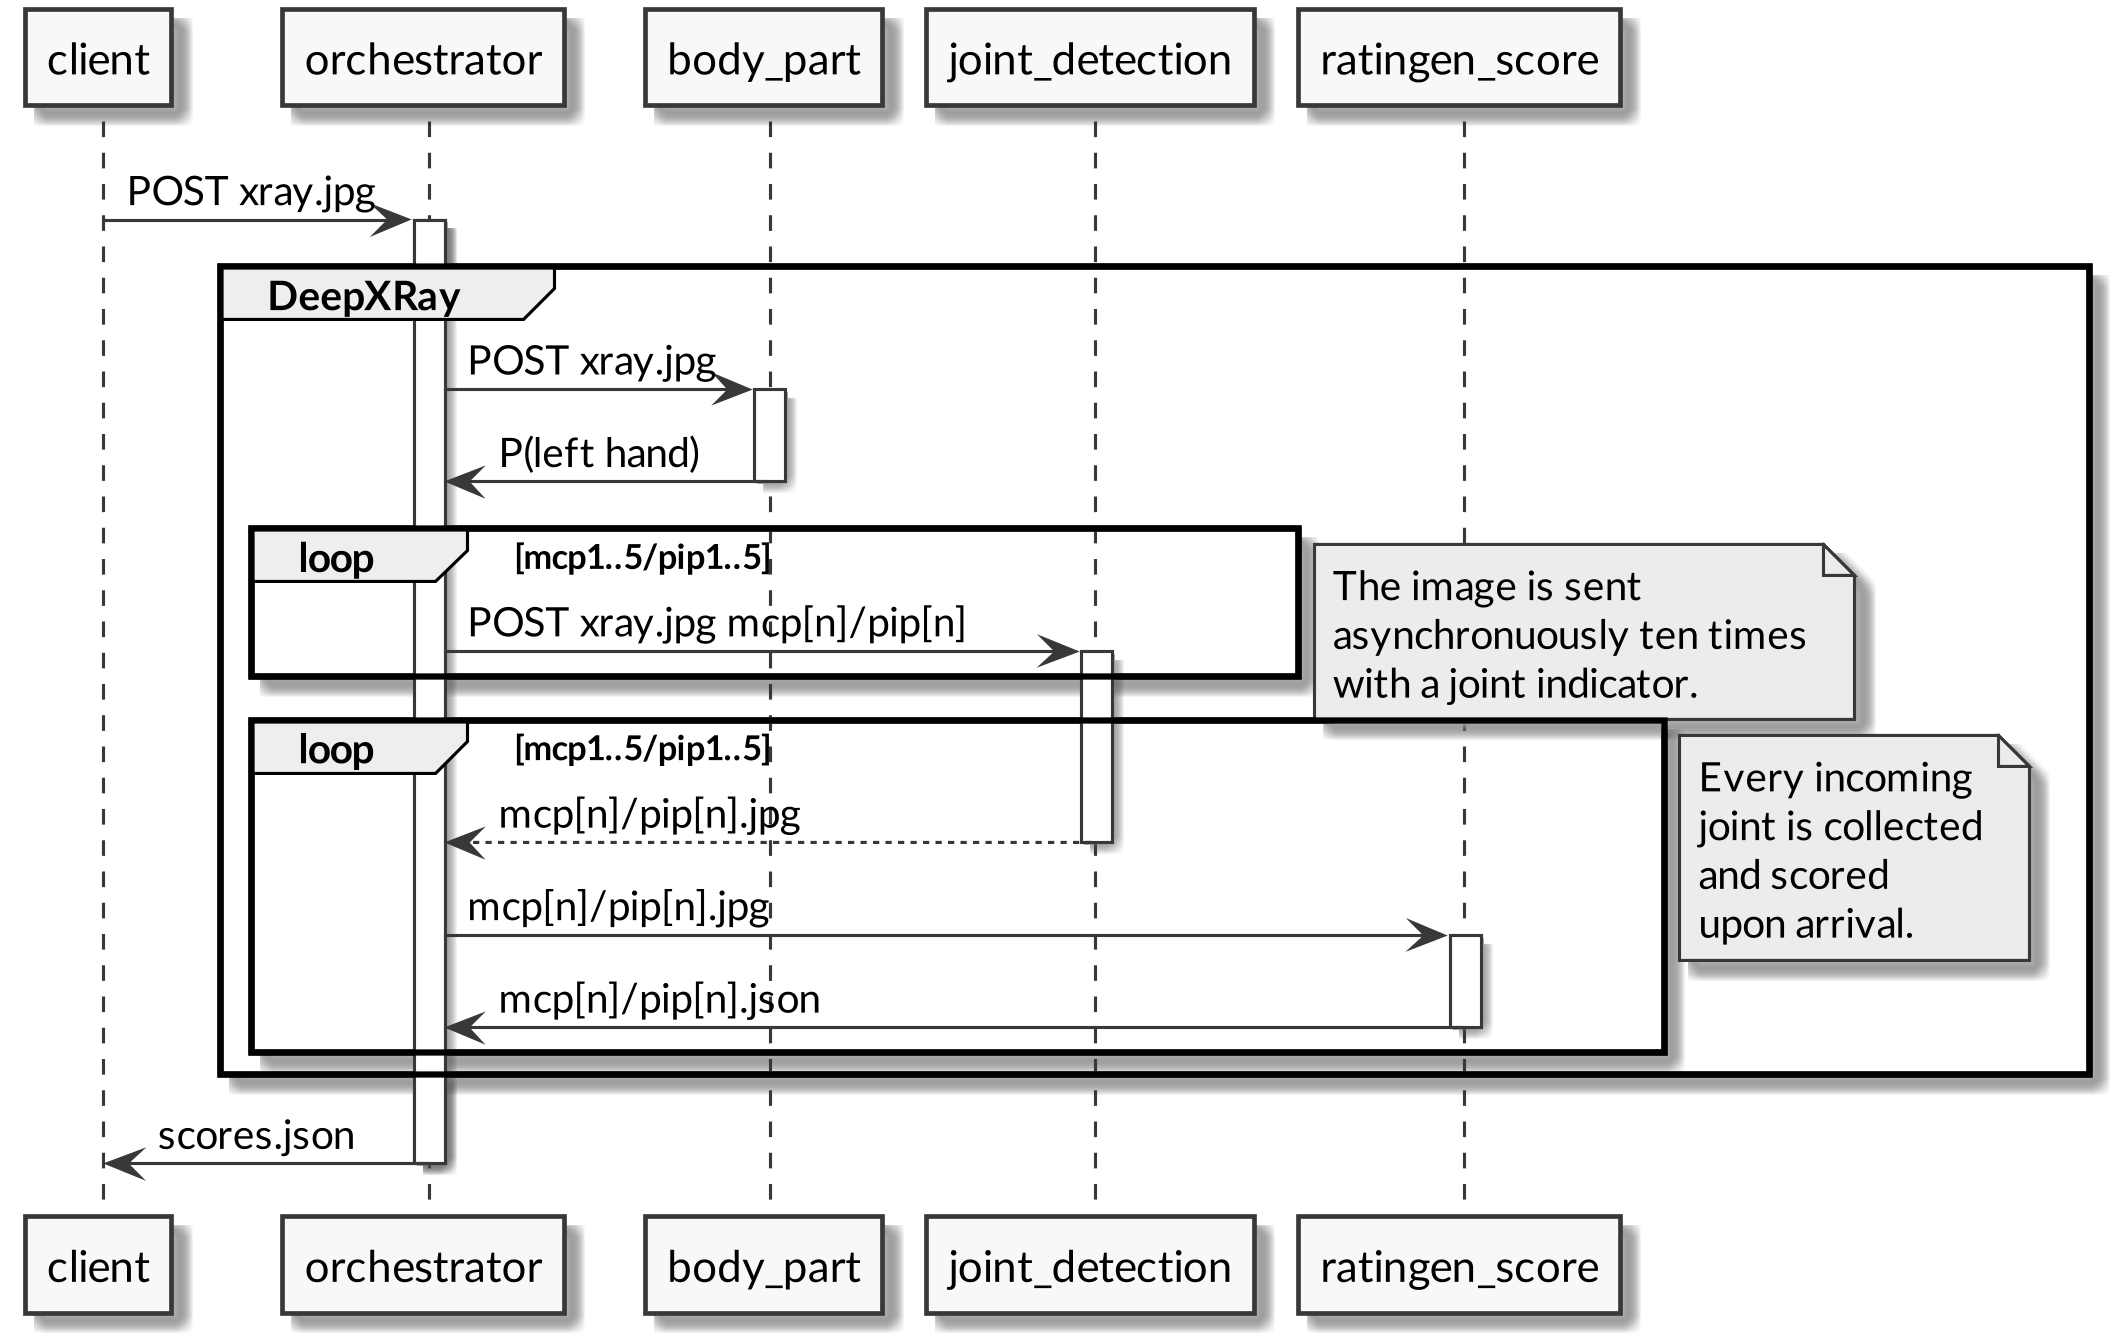
\includegraphics[width=\linewidth]{pics/datenfluss-variante-http-2.png}
    \caption{Datenfluss der Variante 2 (HTTP, synchron und asynchron). Es wird bereits mit dem Scoring begonnen, wenn das erste Gelenk extrahiert ist. (Sequenzdiagramm)}
    \label{fig:datenfluss-variante-http-2}
\end{figure}

Der geänderte Ablauf ist auf \imgref{fig:datenfluss-variante-http-2} ersichtlich. Die Erkennung des Körperteils auf dem Röntgenbild erfolgt wiederum über eine synchrone HTTP-\texttt{POST}-Anfrage an \texttt{body\_part}.

Die Extraktion der Gelenke bei der \texttt{joint\_detection}-Komponente erfolgt jedoch nicht mehr mit einer einzigen Anfrage, deren Antwort synchron abgewartet wird, sondern über eine Anfrage \textit{pro Gelenk}, d.h. es werden zehn Anfragen an \texttt{joint\_detection} gestellt: jeweils mit einem Röntgenbild und dem zu extrahierenden Gelenk. Diese Anfragen werden nebenläufig in einem Unterprozess pro Gelenk abgeschickt.

Sobald ein Unterprozess ein extrahiertes Gelenk von \texttt{joint\_detection} als Antwort erhält, kann damit eine Anfrage für das Scoring an die Komponente \texttt{ratingen\_score} gestellt werden, auf deren Antwort in jedem Unterprozess synchron gewartet wird.

Sind alle zehn Scores eingetroffen, können diese zu einer Antwort für den Client zusammengestellt und an diesen zurückgeschickt werden.

Diese hybride Variante (HTTP asynchron/synchron gemischt) hat Vorteile gegenüber der streng synchronen Variante, löst aber nicht alle Probleme:

\begin{description}
    \item[Vorteile] Es kann bereits mit dem Scoring der Gelenke begonnen werden, wenn das erste Gelenk extrahiert worden ist. So können \texttt{joint\_detection} und \texttt{ratingen\_score} gleichzeitig arbeiten, wodurch die Anfrage des Clients schneller bedient werden kann.
    \item[Nachteile] Das Röntgenbild wird zehnmal statt nur einmal an \texttt{joint\_detection} geschickt. Die Koordination nebenläufiger HTTP-Anfragen ist anspruchsvoller. Ohne zusätzlichen Load-Balancer ist weiterhin nur eine Instanz pro Komponente einsetzbar.
\end{description}

\subsubsection{Variante 3: Messaging zwischen Modellkomponenten}
\label{sec:variante-3-messaging}

Soll die Verarbeitung von Röntgenbildern mit mehreren Instanzen pro Komponente, d.h. parallel vonstatten gehen, wäre mit HTTP ein Load-Balancer pro Komponente nötig. Eine Alternative hierzu stellt das Messaging dar, welches in Abschnitt \secref{sec:integrationsvarianten} vorgestellt worden ist.

Dabei wird die Arbeit nicht an die einzelnen Komponenten erteilt wie bei HTTP (Push), sondern von den einzelnen Komponenten (bzw. deren Instanzen) von einer Queue selbständig abgeholt (Pull). Dies ermöglicht eine parallele Abarbeitung, indem sich die unbeschäftigen Instanzen einer Komponente jeweils neue Arbeit nach dem Round-Robin-Verfahren von der Queue abholen.

\imgref{fig:architektur-variante-queue-1} zeigt eine mögliche Komponentenarchitektur, bei der intern nicht HTTP, sondern Messaging zum Einsatz kommt.\footnote{Hier fällt auf, dass die einzelnen Komponenten jeweils eine Queue \textit{verwenden}, diese aber von keiner der involvierten Komponenten zur Verfügung gestellt wird. Tatsächlich werden die Queues in der Regel von einem \textit{Message-Broker} zur Verfügung gestellt, der aus Gründen der Übersichtlichkeit nicht dargestellt ist. Andererseits gibt es auch Messaging-Lösungen, die ohne Message-Broker-Komponente auskommen, z.B. ZeroMQ.} Bei dieser Variante werden die Komponenten der Reihe nach jeweils paarweise mit einer Queue verbunden, wodurch ein geschlossener Kreis entsteht. Über eine Error-Queue kann der Ablauf im Fehlerfall abgebrochen und als entsprechende Fehlermeldung an den \texttt{orchestrator} weitergegeben werden.

\begin{figure}[tbh]
    \centering
    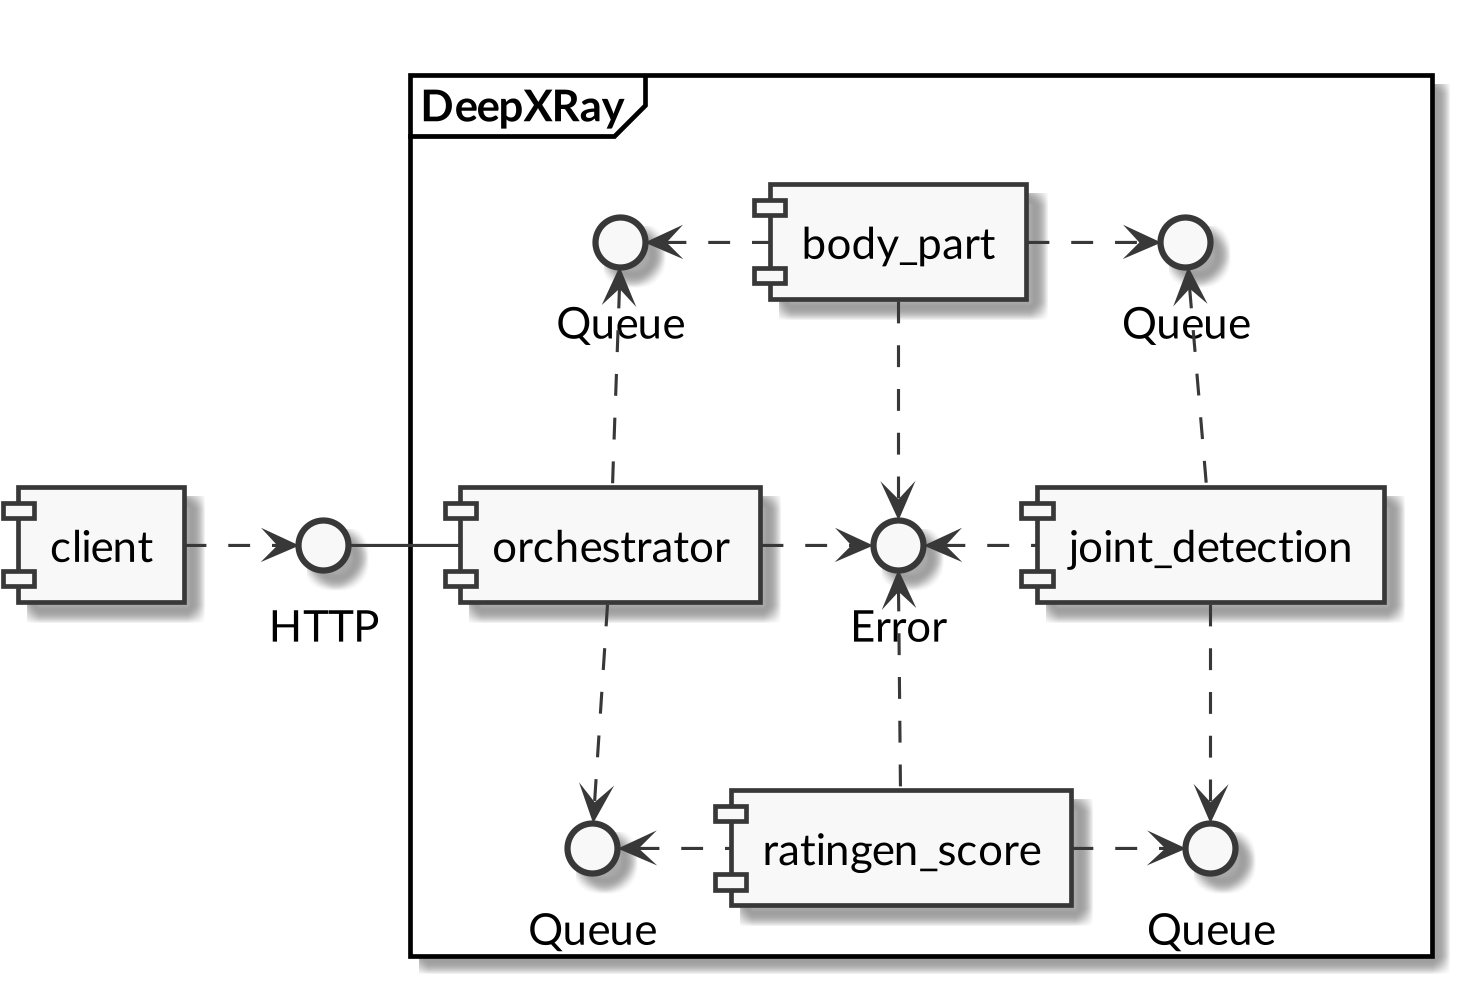
\includegraphics[width=\linewidth]{pics/architektur-variante-queue-1.png}
    \caption{Komponentenarchitektur der Variante 3 (Messaging zwischen den Modellkomponenten). Mithilfe von Message-Queues werden die Komponenten paarweise miteinander verbunden, und bilden so einen Kreis.}
    \label{fig:architektur-variante-queue-1}
\end{figure}

Gegenüber den ersten beiden Varianten (HTTP rein synchron und hybrid, d.h. asynchron/synchron) ändert sich der Ablauf grundlegend (siehe \imgref{fig:datenfluss-variante-queue-1}). Der \texttt{orchestrator} empfängt wiederum das Röntgenbild per HTTP vom Client. Er reicht dieses über eine Queue weiter an die Komponente \texttt{body\_part}. Hier gibt der \texttt{orchestrator} die Kontrolle über die Weiterverarbeitung ab.

Wird auf dem Röntgenbild eine linke Hand erkannt, reicht \texttt{body\_part} das Röntgenbild zur Extraktion der Gelenke an \texttt{joint\_detection} weiter, wiederum über eine Queue. Hier werden die zehn Gelenke der Reihe nach extrahiert. Jedes extrahierte Gelenk wird sogleich über eine weitere Queue an \texttt{ratingen\_score} weitergegeben. Es kann wiederum mit dem Scoring begonnen werden, wenn die Extraktion der Gelenke noch in Gang ist.

Die Scores werden von \texttt{ratingen\_score} über eine Queue an den \texttt{orchestrator} weitergereicht. Treten bei der Extraktion oder beim Scoring Fehler auf, werden diese über eine Error-Queue an den \texttt{orchestrator} gemeldet. Dieser braucht pro ursprünglich eingegangenem Request (Röntgenbild) zwei Queues zu beobachten: Die ermittelten Scores und die gemeldeten Fehler. Insgesamt müssen pro Vorgang zehn Nachrichten beim \texttt{orchestrator} eingehen, seien dies Scores oder Fehlermeldungen. Sind diese alle eingetroffen, kann der Client bedient werden.

\begin{figure}[tbh]
    \centering
    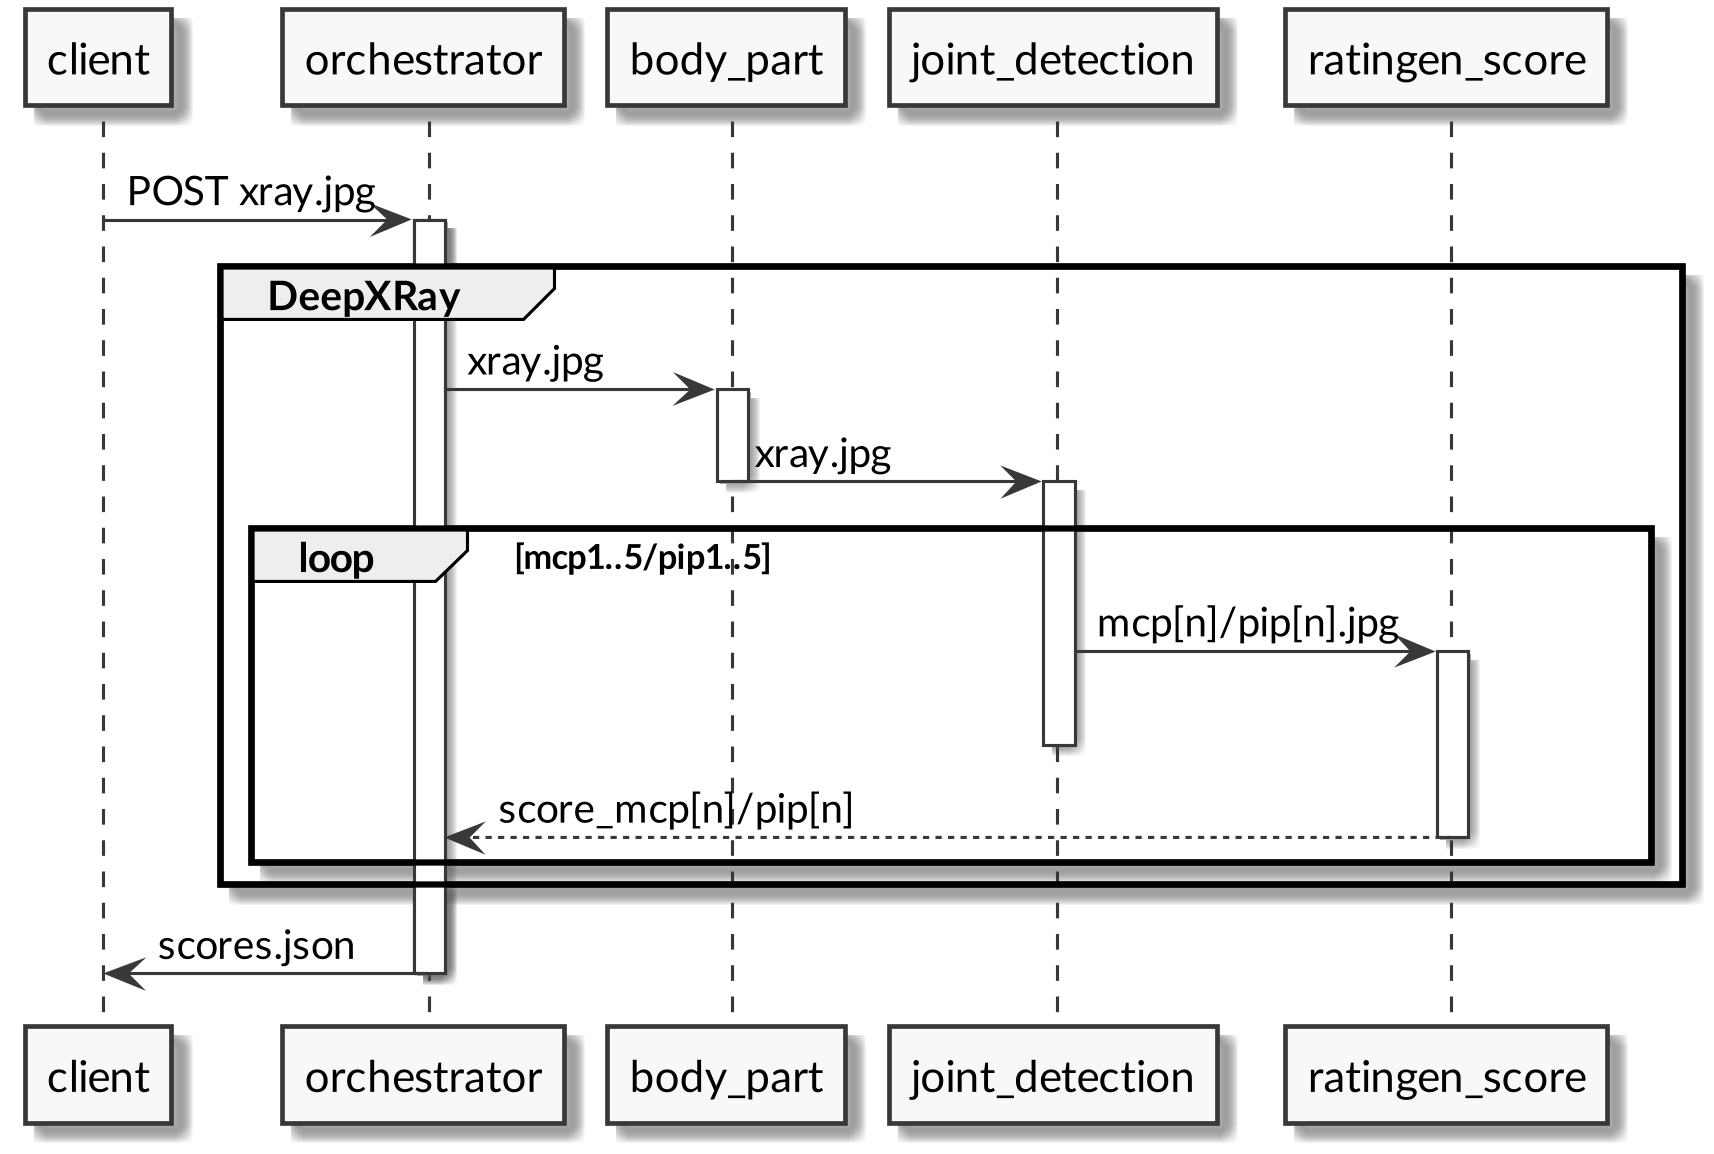
\includegraphics[width=\linewidth]{pics/datenfluss-variante-queue-1.png}
    \caption{Datenfluss der Variante 3 (Messaging zwischen den Modellkomponenten). Die Anfragen werden via Message-Queue von Komponente zu Komponente weitergereit. (Sequenzdiagramm)}
    \label{fig:datenfluss-variante-queue-1}
\end{figure}

Die asynchrone Verarbeitung über Message-Queues ermöglicht es, dass alle drei Modellkomponenten mit beliebig vielen Instanzen ausgeführt werden können, was die Verarbeitungsgeschwindigkeit bis zu einem gewissen Grad erhöht. Das «Einsammeln» der Ergebnisse wird über diese asynchrone Abarbeitung jedoch erschwert, zumal zu einem bestimmten Zeitpunkt die Nachrichten verschiedener Anfragen in den Queues hängen können. Der \texttt{orchestrator} benötigt darum einen Mechanismus, um die  eintreffenden Nachrichten einer ursprünglichen HTTP-Anfrage zuordnen zu können. Andernfalls könnte der Client mit seiner Antwort Informationen bekommen, die zu anderen Anfragen gehören.

Dieses Problem kann mit einem \textit{Correlation Identifier} gelöst werden \cite[S. 163-169]{enterprise-integration-patterns}. Hierzu wird jeder Anfrage eine eindeutige Identifikation zugewiesen. Dies kann eine fortlaufende Nummerierung sein, oder aber ein generierter Zufallswert. Wichtig ist, dass dieser Wert im gegebenen Kontext eindeutig ist. Die Message wird mit diesem Correlation Identifier ausgestattet und für Folgenachrichten übernommen. Sammelt der \texttt{orchestrator} die eingehenden Nachrichten von den beiden Queues ein, kann er diese über den Correlation Identifier dur urpsprünglichen Anfrage zuordnen.

Diese auf Messaging basierte Architekturvariante stellt in vielerlei Hinsicht eine Verbesserung gegenüber den beiden HTTP-Varianten dar, bringt aber auch neue Probleme mit sich:

\begin{description}
    \item[Vorteile] Über den Messaging-Ansatz wird eine parallele Abarbeitung ohne zusätzliche Load-Balancer ermöglicht.
    \item[Nachteile] Das asynchrone «Einsammeln» von Nachrichten und deren Zuordnung zu den ursprünglichen Client-Anfragen erfordert einen zusätzlichen Mechanismus (Correlation Identifier). Die dezentrale Kommunikation zwischen den Modellkomponenten ist komplizierter, da es mehr Kommunikationspaare gibt.
\end{description}

Zudem funktioniert der beschriebene Ansatz nur für das unmittelbar gegebene Problem: das Scoring von (linken) Händen, wobei immer genau zehn Gelenke von Interesse sind. Sollen in Zukunft auch die Röntgenbilder anderer Körperteile verarbeitet werden, etwa Becken mit zwei Hüftgelenken, funktioniert dieser Ansatz nicht mehr. Das Problem ist, dass der \texttt{orchestrator} nicht erfährt, welches Körperteil auf einem Röntgenbild dargestellt wird, und so nicht wissen kann, wie viele Scores (oder Fehlermeldungen) er einzusammeln hat.

\subsubsection{Variante 4: Messaging, synchron und asynchon}
\label{sec:variante-4-messaging}

Um für zukünftige Erweiterungen von anderen Körperteilen gerüstet zu sein, muss der \texttt{orchestrator} wissen, welches Körperteil auf einem Röntgenbild dargestellt ist, um so die richtige Anzahl an Scores bzw. Fehlermeldungen erwarten zu können. Darum wird \texttt{body\_part} gegenüber der Variante 3 aus dem Kreis der vier Komponenten entfernt und synchron an den \texttt{orchestrator} gekoppelt. Die Komponentenarchitektur ist auf \imgref{fig:architektur-variante-queue-2} ersichtlich.

\begin{figure}[tbh]
    \centering
    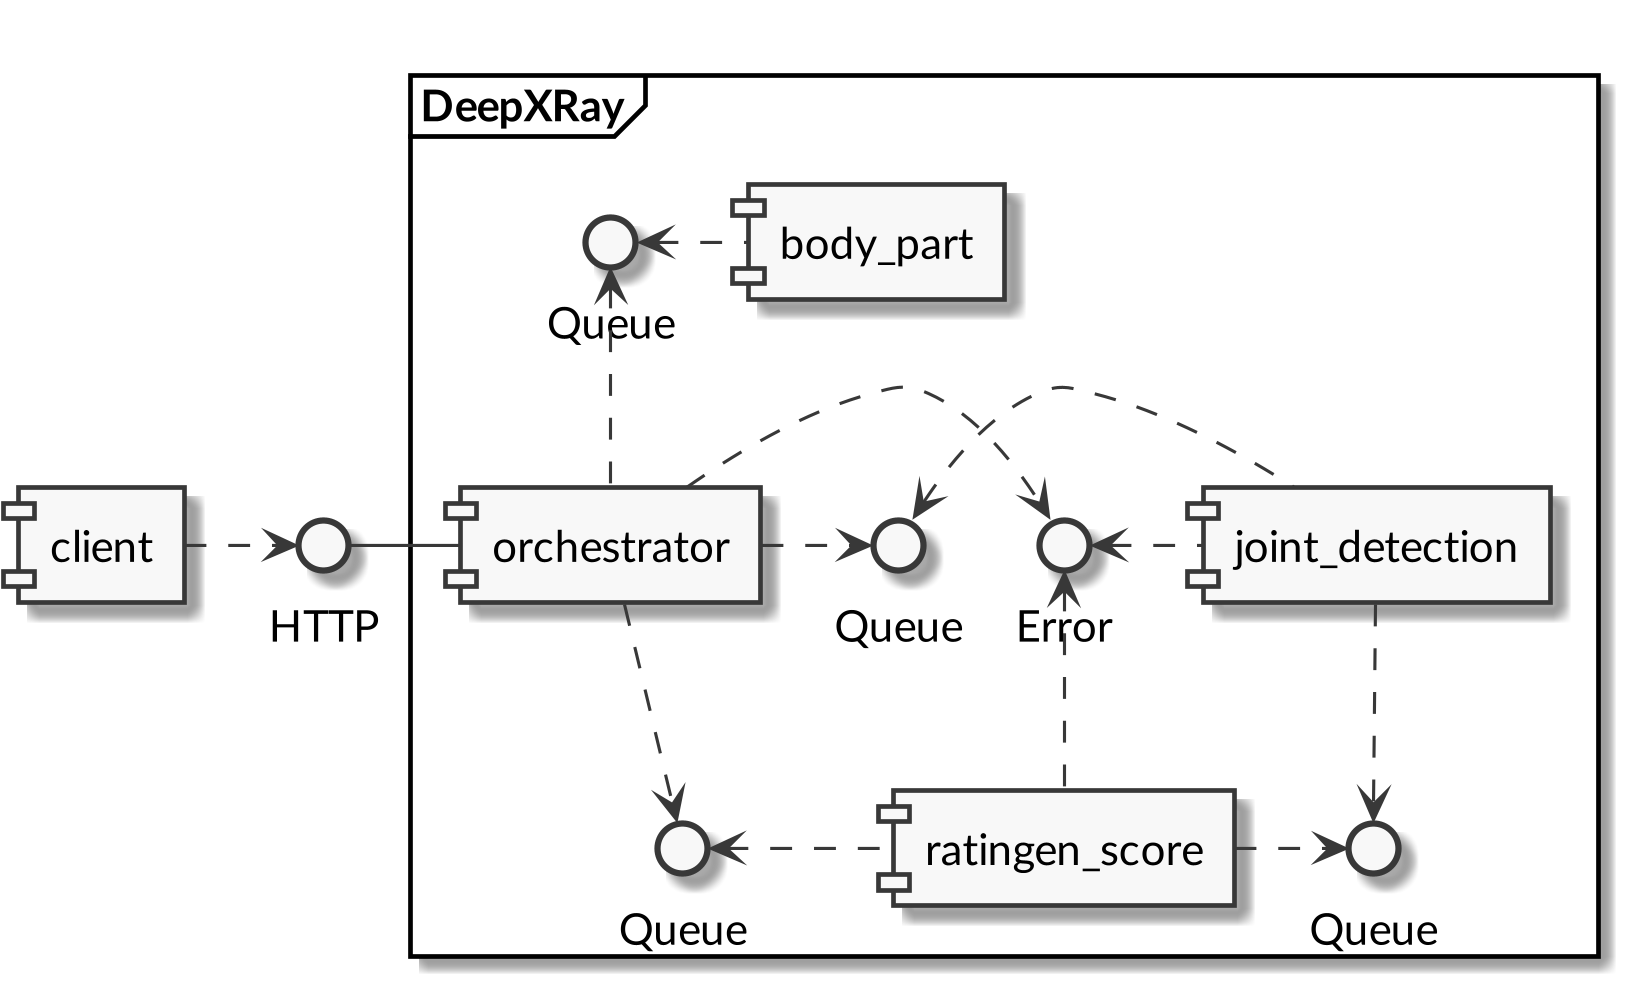
\includegraphics[width=\linewidth]{pics/architektur-variante-queue-2.png}
    \caption{Komponentenarchitektur der Variante 4 (Messaging, synchron und asynchron). Die \texttt{body\_part}-Komponente ist synchron, die anderen Modellkomponenten sind asynchron angebunden.}
    \label{fig:architektur-variante-queue-2}
\end{figure}

Obwohl die Kommunikation zwischen \texttt{body\_part} und dem \texttt{orchestrator} synchron abläuft, soll dennoch eine Message-Queue als Schnittstelle zwischen diesen Komponenten dienen. Dies hat den Vorteil, dass \texttt{body\_part} mit mehreren Instanzen gleichzeitig betrieben werden kann, die sich die Workloads abwechselnd von der Queue holen, die nicht nur als Übertragungsmedium, sondern auch als Load-Balancer fungiert.

Der Datenfluss ändert sich dabei gegenüber der vorherigen Messaging-Variante beträchtlich (siehe \imgref{fig:datenfluss-variante-queue-2}). Das Körperteil wird ‒ wie bei den beiden HTTP-Varianten ‒ synchron detektiert. Wurde eine linke Hand erkannt, gibt der \texttt{orchestrator} ‒ und nicht \texttt{body\_part}! ‒ die Extraktionen in Auftrag. Da hier nun Messaging zum Einsatz kommt, können zehn entsprechende Nachrichten auf der Queue publiziert werden, von der \texttt{joint\_detection} liest.

Extrahierte Gelenke werden über eine weitere Queue an \texttt{ratingen\_score} weitergeleitet. Scheitert die Extraktion oder das Scoring, kann dies über eine Error-Queue an den \texttt{orchestrator} gemeldet werden. Da dieser die Extraktion der Gelenke in Auftrag gegeben hat, ist diesem die Anzahl der zu erwartenden Nachrichten bekannt. Sind diese Nachrichten eingetroffen, kann er den Client damit bedienen.

\begin{figure}[tbh]
    \centering
    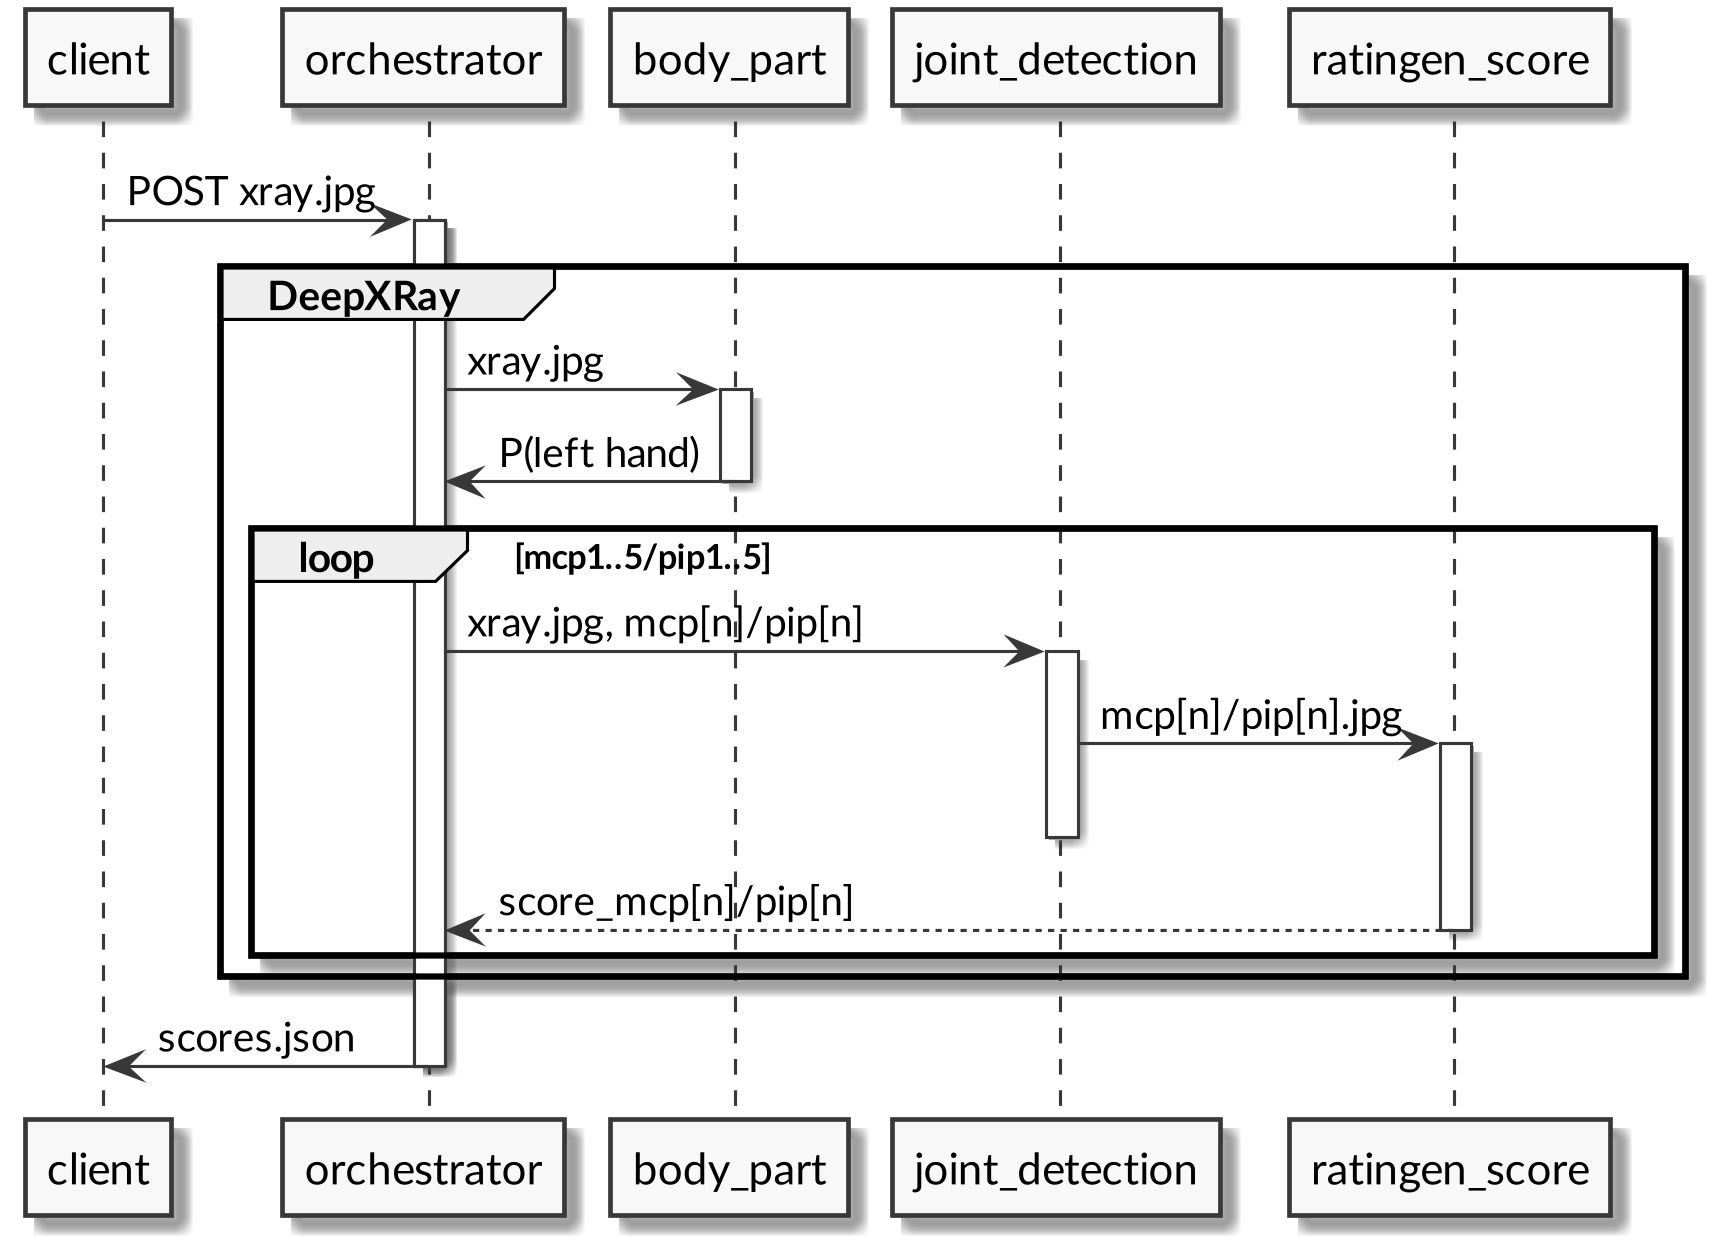
\includegraphics[width=\linewidth]{pics/datenfluss-variante-queue-2.png}
    \caption{Datenfluss der Variane 4 (Messaging, synchron und asynchron). Die Modellkomponente \texttt{body\_part} wird synchron, die Modellkomponenten \texttt{joint\_detection} und \texttt{ratingen\_score} werden asynchron angebunden. (Sequenzdiagramm)}
    \label{fig:datenfluss-variante-queue-2}
\end{figure}

Diese Variante kombiniert die Vorteile der synchronen Erkennung des Körperteils mit den Vorteilen der nebenläufigen Extraktion und dem Scoring der Gelenke:

\begin{description}
    \item[Vorteile] Die Gelenke können nebenläufig extrahiert und gescored werden, was eine höhere Verarbeitungsgeschwindigkeit ermöglicht. Mithilfe von Messaging können die Komponenten mit mehreren Instanzen parallel betrieben werden. Zudem funktioniert die Architektur auch dann noch, wenn andere Körperteile als linke Hände (mit einer anderen Anzahl relevanter Gelenke) verarbeitet werden sollen.
    \item[Nachteile] Das «Einsammeln» der Nachrichten erfordert ‒ gleich wie die vorherige Mes\-sag\-ing-Variante ‒ einen Correlation Identifier. Der \texttt{orchestrator} hat noch mehr Kommunikationsaufgaben. Zudem wird das Röntgenbild einmal pro Gelenk publiziert, nicht einmal für alle zehn Gelenke.
\end{description}

\subsubsection{Entscheidung}

Jede Variante bietet Vorteile gegenüber ihrem Vorgänger: Variante 1 (HTTP, synchron) arbeitet streng sequenziell. Variante 2 (HTTP, asynchron/synchron) kann bereits mit dem Scoring beginnen, wenn die Extraktion noch nicht abgeschlossen ist. Variante 3 (Mes\-sag\-ing zwischen Modellkomponenten) ermöglicht die Ausführung mehrerer Instanzen eines Modells. Variante 4 (Messaging, synchron und asynchron) lässt sich darüber hinaus am besten erweitern. Trotz der Nachteile von Variante 4 ‒ Notwendigkeit eines Correlation Identifiers, mehrfache Publikation des Röntgenbilds (einmal pro Gelenk), verschiedenartige Kommunikationsaufgaben (synchron und asynchron) ‒ ist sie die flexibelste und am besten erweiterbare Variante.

Der Prototyp soll darum gemäss Variante 4 (Messaging, synchron und asynchron) umgesetzt werden.

\subsection{Austauschbarkeit von Modellen}
\label{sec:austauschbarkeit-von-modellen}

Die Modelle ‒ oder Modellkomponenten ‒ müssen gemäss Projektauftrag (siehe \secref{sec:erwartetes-resultat}) austauschbar sein. Für diese Anforderung gibt es verschiedene Lösungsansätze.

Ein Lösungsansatz wäre die Austauschbarkeit auf Modellebene. Hierzu wurden entsprechende Formate ‒ TensorFlow SavedModel und ONNX ‒ im Abschnitt \secref{sec:modellformate} vorgestellt. Die bestehenden Modelle lassen sich jedoch nicht einfach in eines dieser Formate konvertieren. Zudem ist die Wahl eines dieser Formate noch keine Garantie für Vorwärtskompatibilität in einigen Jahren. Ändert sich die Modellspezifikation (Inputs, Outputs) nur geringfügig, ist die Austauschbarkeit auf Modellebene bereits nicht mehr gegeben. Die Austauschbarkeit von Modellen (oder Modellkomponenten) über die Modelldatei ist somit für das vorliegende Projekt keine Option.

Statt die Modelle selber austauschbar zu machen, und so Änderungen an ihren Inputs und Outputs für längere Zeit zu verunmöglichen, können die Modell\textit{komponenten} austauschbar gemacht werden. Hierfür wird eine API spezifiziert, an die sich die Modellkomponenten halten müssen. Da für den Prototyp Messaging zum Einsatz kommen soll (siehe \secref{sec:variante-4-messaging}), ist diese API einerseits über das Nachrichtenformat, andererseits über die verwendete Messaging-Technologie (z.B. AMQP oder MQTT) zu definieren.

Da die verwendeten Modelle auf verschiedenen Versionen von TensorFlow basieren und mit unterschiedlichen High-Level-APIs (tflearn, Keras) erstellt worden sind, können diese nicht in der gleichen Laufzeitumgebung ausgeführt werden.

Mit virtuellen Python-Umgebungen ist es möglich, auf dem gleichen Rechner verschiedene Python-Versionen mit den dazugehörigen Libraries und Frameworks auszuführen. Mit dem Modul \texttt{venv} \footnote{\url{https://docs.python.org/3/library/venv.html} (abgerufen am 11.05.2020)} können verschiedene virtuelle Python-Um\-ge\-bung\-en auf einem Rechner erstellt werden, die auf der installierten Python-Version basieren.

Da die verwendeten Frameworks/Libraries jedoch nicht zu den neuesten Versionen von Python kompatibel sind, müssten auch verschiedene Versionen des Python-In\-ter\-pret\-ers installiert werden können. Das Modul \texttt{pyenv}\footnote{\url{https://github.com/pyenv/pyenv} (abgerufen am 11.05.2020)} unterstützt dies. Diese Variante ist aber für den Produktiveinsatz riskant, zumal mehrere ältere Versionen des Python-Interpreters auf dem gleichen System laufen, und so den Angriffsvektor dieses Systems vergrössern.\footnote{Das gestellte Problem ist ja, dass aufgrund von Inkompatibilitäten auf Ebene Libraries/Frameworks ältere Versionen von Python verwendet werden müssen. Das Modell \texttt{ratingen\_score} wurde etwa mit Python 3.5 erstellt ‒ eine Version, die nur noch bis am 13.09.2020 Updates erhalten soll (\url{https://devguide.python.org/\#branchstatus}, abgerufen am 11.05.2020).}

Container ermöglichen nicht nur die Installation praktisch beliebiger (älterer) Versionen von Python, sondern auch die Isolation dieser Umgebungen. So können ältere Versionen verwendet werden, ohne die Sicherheit des zugrundeliegenden Systems zu beeinträchtigen. Container-Runtimes wie Docker ermöglichen es zudem, Ports für die Kommunikation zwischen dem Container und dem zugrundeliegenden System bzw. Ports zwischen einzelnen Containern per Konfiguration zu definieren.

Werden die Modellkomponenten als Container umgesetzt, können sie auf Basis ihrer Schnittstelle ‒ Messaging-Format, Messaging-Protokoll und Port ‒ austauschbar gemacht werden. Welche Libraries, Frameworks, Python-Versionen und Modellformate dabei zum Einsatz kommen, ist für die Umsysteme nicht relevant.

Die Austauschbarkeit von Modellkomponenten soll darum mithilfe von Containern gewährleistet werden.

\subsection{Parallelisierung ‒ Nebenläufigkeit}

Der Projektauftrag nennt das «Verteilen über mehrere GPUs» als Anforderung (siehe \secref{sec:erwartetes-resultat}). Dieser ist nicht ohne Weiteres nachzukommen, da zur Ausführung eines Modells auf einer GPU dieses komplett in den Speicher derselben geladen werden muss. Da für die Gelenkextraktion nicht nur ein Modell, sondern zehn verschiedene Modelle in den Speicher geladen werden müssen, dürfte eine Vielzahl von GPUs nötig sein, um die Ausführung damit zu beschleunigen. Ein solches Setup steht für die Entwicklung nicht und für den Produktiveinsatz wohl kaum zur Verfügung.\footnote{Der Cloud-Anbieter Exoscale, der auch Hosting in der Schweiz anbietet, was für sensible Patientendaten wie Röntgenbilder auch erforderlich ist, verlangt für eine Instanz mit vier GPUs 2.28 € pro Stunde, d.h. bis zu 1696.32 € pro Monat.}

Auch wenn dieses optimale, auf GPUs basierende Setup vorerst keine Option ist, ist die parallele Ausführung der verschiedenen Modelle für eine akzeptable End-to-End-Perfomance unbedingt erforderlich ‒ und darum auch für die Architekturdiskussion (siehe \secref{sec:architekturvarianten}) eine grundlegende Anforderung.

Doch genügt eine geeignete Architektur, um Parallelisierung zu gewährleisten? Um diese Frage beantworten zu können, lohnt sich ein genauerer Blick auf die Begriffe \textit{Nebenläufigkeit} (engl. \textit{concurrency}) und \textit{Parallelität} (engl. \textit{parallelism}).

Die Begriffe werden oft synonym gebraucht, haben aber unterschiedliche Bedeutungen ‒ die zugegebenermassen in einer Welt mit allgegenwärtigen Multicore-Systemen kaum noch erfahrbar sind.

Doch der Reihe nach: Rob Pike, einer der Schöpfer der Programmiersprache Go, definiert die beiden Begriffe folgendermassen: \textit{«Concurrency and Parallelism are not the same thing. \[...\] Concurrency is \[...\] the composition of independently executing processes. Parallelism, on the other hand, ist the simultaneous execution of multiple things. \[...\] One is really about structure (concurrency), and one is about execution (parallelism).»}\footnote{Nebenläufigkeit und Parallelität sind nicht das Gleiche. Nebenläufigkeit ist die Komposition unabhängig voneinander ablaufender Prozesse. Parallelität hingegen ist die gleichzeitige Ausführung mehrerer Dinge. Bei einem geht es um die Struktur (Nebenläufigkeit), beim anderen geht es um die Ausführung (Parallelität). (Übersetzung des Autors)} \cite[ab 1:16]{concurrency-is-not-parallelism}.

Joe Armstrong, der 2019 verstorbene Schöpfer der Programmiersprache Erlang, geht genauer auf die Hardware-Aspekte dieser Konzepte ein: \textit{«In everyday language, words like concurrent, simultaneous, and parallel mean almost the same thing. But in programming languages, we need to be more precise. In particular, we need to distinguish between concurrent and parallel programs. If we have only a single-core computer, then we can never run a parallel program on it. This is because we have one CPU, and it can do only one thing at a time. We can, however, run concurrent programs on a single-core computer. The computer time-shares between the different tasks, maintaining the illusion that the different tasks run in parallel.»}\footnote{In der Alltagssprache bedeuten Wörter wie «nebenläufig», «gleichzeitig» und «parallel» fast das Gleiche. Bei Programmiersprachen muss man aber präziser sein. Besonders «nebenläufig» und «parallel» muss man voneinander unterscheiden. Hat man nur einen Single-Core-Computer, kann man niemals ein paralleles Programm auf ihm laufen lassen. Das liegt daran, dass man nur eine CPU hat, und diese kann nur eine Sache zur gleichen Zeit machen. Wir können jedoch ein nebenläufiges Programm auf einem Single-Core-Computer ausführen. Der Computer wechselt zwischen den verschiedenen Aufgaben hin und her, und hält die Illusion aufrecht, mehrere Aufgaben parallel abzuarbeiten. (Übersetzung des Autors)} \cite[S. 8]{programming-erlang}.

Parallelisierung erreicht man also dadurch, indem man ein nebenläufiges Programm auf Hardware mit mehreren CPU-Kernen bzw. mehreren CPUs laufen lässt. Ein nebenläufiges Programm muss so strukturiert sein, dass es potenziell mit mehreren Vorgängen gleichzeitig zurecht kommt. Eine solche Struktur wurde in der Architekturdiskussion erarbeitet (siehe \secref{sec:variante-4-messaging}). Wird der Prototyp entsprechend umgesetzt, ist Parallelität praktisch automatisch gegeben, zumal heute kaum noch Rechner mit nur einem CPU-Kern im Einsatz sind.

\clearpage
